\documentclass[11pt]{article}
\usepackage{ROSPINCanSat, lipsum, xcolor}
\cansatstyle

\title{Guidelines for the Critical Design Report
}
\author{Team: ROSPIN}
\date{January 22, 2024}

\begin{document}

\cansattitle


%%%%%%%%%% INTRO PAGE - DELETE BEFORE SUBMISSION %%%%%%%%%%%

The process of building a satellite is very complex and costly. That is why, in a real satellite mission, before, during, and after the satellite is built, these documents provide detailed information about the satellite being developed and ensure that it complies with all the requirements regarding the mission and the launch environment.

The process of designing and building a CanSat is much simpler than the one followed for a satellite. Nevertheless, we believe that exposing students to good engineering procedures will be very beneficial for their educational experience.

These guidelines provide information about the expected content of each \textbf{Critical Design Report (CDR)} chapter. 
This information will ensure that your work is aligned with your mission goals and can help us identify possible problems at an early stage. 
It will also allow us to determine that your CanSat will be able to fly according to the mechanical and safety requirements.

Attached to this document, there is a sample design document with a given structure that you can use to describe all the aspects of your CanSat project. 
Your report should be no longer than \textbf{30 pages}, not including appendices and references. Appendices should be used for detailed information 
to keep the document's main body as concise as possible. This detailed information may be, e.g., details of scientific background, technical drawings, or 
component datasheets. The documentation should be written clearly and concisely, allowing a person who does not know the experiment to understand its purpose and design.

The design document should provide the JURY with all the relevant information regarding the experiment. 
During all experiment phases, the design document is the only documentation for describing the experiment in detail. 
Additional sections can be added by the team if appropriate. However, the present sections should be included in your CDR for reference. The design document will be the main evaluating criteria for the Romanian CanSat and Rocketry Competition jury.

\vspace{3cm}
{\Large{\textbf{Note:} Do not include this page in your Report!}}
%%%%%%%%%% END OF INTRO PAGE - DELETE BEFORE SUBMISSION %%%%%%%%%%%


\newpage

\tableofcontents
\pagestyle{plain}

\newpage





% First section
\section{Progress report}
% Write the progress report here

\subsection{New progress statement for the team profile}
% Here comes the content regardin the new progress statement for the team profile

\subsection{Tasks list}
% Here comes the content regardin the tasks list

\subsection{Detailed project status}
% Here comes the content regardin the detailed project status




% 2nd section
\section{Introduction}
% Write the introduction text here

\subsection{Purpose of the mission}
% Here comes the content regardin the purpose of the mission.

\subsection{Team organisation and roles}
% Here comes the team organisation and roles description content.

\subsection{Mission objectives}
% Here comes the text regarding the mission objectives.




% 3rd section
\section{CanSat description / Payload description}
% Write the CanSat description text here for the CanSat challenge
% or the Payload escription text here for the Rocketry challenge

\subsection{Mission overview}
% Here comes the text regarding the mission overview.

\subsection{Mechanical / structural design}
% Here comes the text regarding the mechanical and structural design.
\begin{enumerate}
\item \textbf{Mechanical Design:} The CanSat is made of carbon fiber/ alluminum alloy because of their mechanical properties such as low weight, high durability and high tolerances in thermal expansion. The structure was designed to maintain a certain position while mid-air and to withstand the stress of launch and landing. It comes with a removable top and bottom to facilitate access inside. The components are attached to the structure with screws, nuts and mounts to assure stability during the mission.
\vspace{0.25cm}
\item \textbf{Components:} Components used for building the CanSat include: a main board, sensors, a video camera, a battery and a GPS module. The main board contains the microcontroller which collects the data from the sensors and sends it to the ground station via it’s communication module. The sensors include: a temperature sensor, a CH4 sensor, a N2 sensor, a CO2 sensor and an altimeter which measures both pressure and altitude. The GPS module registers the current position of the CanSat. The video camera takes frames of the surface below to be processed afterwards at the ground station. The battery provides power to the CanSat during flight. The list of components stands as it follows:

\begin{itemize}
\item \textbf{Microcontroller:} Raspberry PI Zero
\item \textbf{Temperature sensor:} sensor DS18B20
\item \textbf{CH4 sensor:} sensor MQ-4
\item \textbf{N2 sensor:} sensor MiCS-5524
\item \textbf{CO2 sensor:} sensor MQ-9
\item \textbf{Altimeter:} sensor BMP-388
\item \textbf{GPS Module:} GPS GY-NEO6MV2 module
\item \textbf{Communication module:} already integrated in main board
\item \textbf{Gyroscope:} sensor MPU6050
\item \textbf{Video Camera:} OV5647 video camera
\item \textbf{Rechargable battery:} portable power bank
\end{itemize}

\item \textbf{Placement:} The main board is attached to the top of the CanSat structure with the sensors located adjacent to it. The battery is attached to a side of the CanSat while the camera is attached to the opposite side of it. The structure was designed to maintain balance during flight, to minimize the weight and to provide space for the components and for further human intervention.
\vspace{0.25cm}
\item \textbf{Drawings:} This is a mechanical drawing of the CanSat structure in which we have emphasized on the placement of the major components.

\begin{figure}[h]
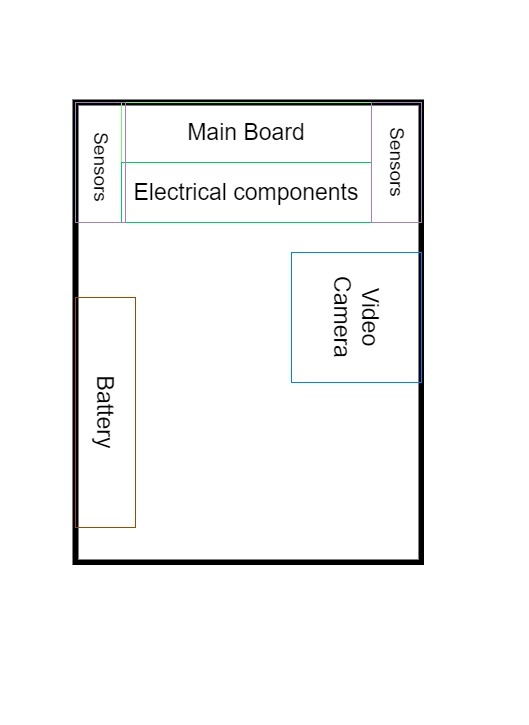
\includegraphics[width=8cm]{Component_placement}
\centering
\end{figure}

\item \textbf{Explanation:} The main board contains the microcontroller which collects the data from the sensors and sends it to the ground station via it’s communication module. The temperature sensor measures the temperature of the environment, the CH4 sensor, the N2 sensor and the CO2 sensor measures the atmospheric gasses in the air and the altimeter measures both pressure and altitude at the CanSat’s point. The GPS module registers the current position of the CanSat. The video camera takes frames of the surface below to be processed afterwards at the ground station. The battery provides power to the CanSat during flight.

\end{enumerate}

\subsection{Electrical design}
% Here comes the text regarding the electrical design.
\begin{enumerate}
\item \textbf{Electrical Interface:}
\item \textbf{RF Link:}
\item \textbf{Power Budget:}
\item \textbf{Power Consumption and Duration:}
\item \textbf{Battery:} 

\begin{figure}[h]
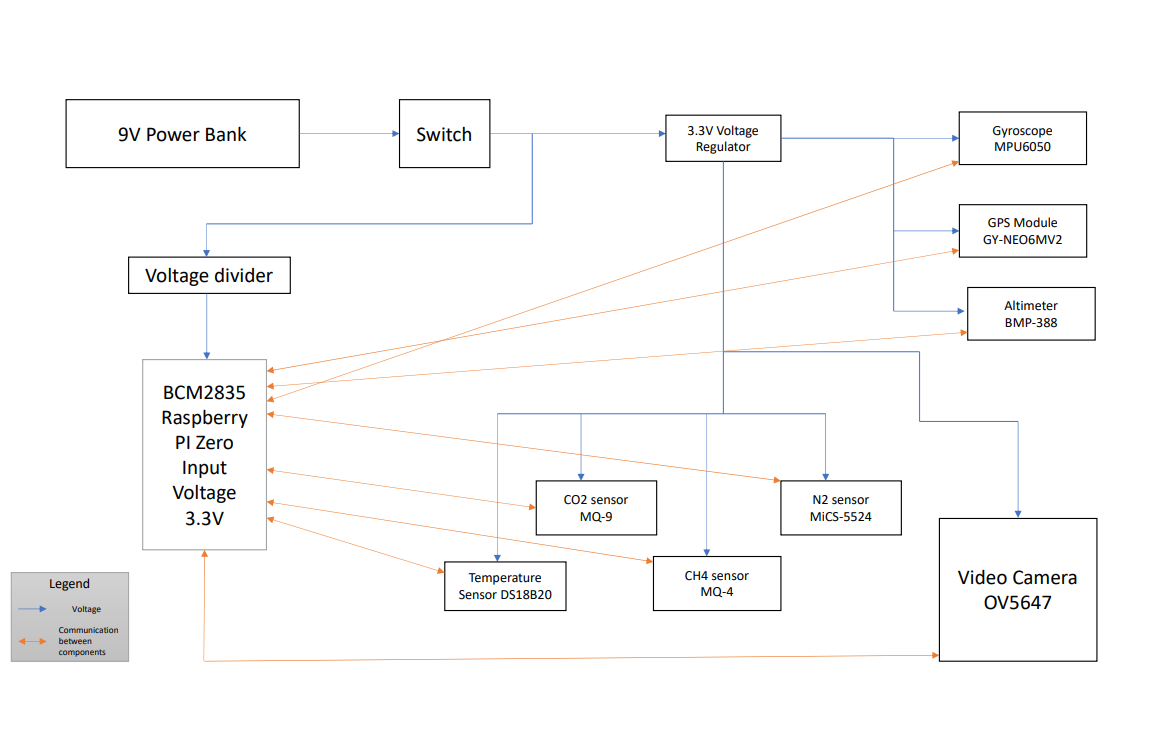
\includegraphics[width=15cm]{Schema_electrica}
\centering
\end{figure}
\end{enumerate}

\subsection{Software design}
% Here comes the text regarding the software design.

\subsection{Recovery system}
% Here comes the text regarding the recovery system.
\begin{enumerate}
\item \textbf{Description:} The Recovery System was designed to assure a safe landing and a controlled descent of the CanSat. It consists of a parachute that is attached to the CanSat structure using a harness that is made of nylon fibres and that wad designed to resist the velocity and the force applied during descent. The parachute is deployed at a certain altitude.
\vspace{0.25cm}
\item \textbf{Method of attachment:} The parachute is attached to the CanSat structure using a harness thar is made of nylon fibres. The harness is connected to the structure itself with screws and PVC collars providing a stable attachment for the recovery system
\vspace{0.25cm}
\item \textbf{Expected flight time:} The CanSat estimated time flight is … in which it reaches it's maximum altitude and reaches the ground by using the recovery system

\end{enumerate}

\subsection{Ground support equipment}
% Here comes the text regarding the ground support equipment.

% section only for the Rocketry Challenge
% \section{Rocket Description}

% \subsection{Rocket Mission overview}
% % Here comes the text regarding the mission overview.

% \subsection{Rocket's mechanical / structural design}
% % Here comes the text regarding the mechanical and structural design.

% \subsection{Rocket's recovery system}
% % Here comes the text regarding the recovery system.


% 4th section
\section{Project planning}
% Write about the project planning here

\subsection{Time schedule of the project preparation}
% Here comes the text regarding the time schedule.

\subsection{Resource estimation}
% Here comes the text regarding the resource estimation.

\subsubsection{Budget}
% Here comes the text regarding the budget.
\begin{center}
	\begin{tabular}{|c|c|}
		\hline
		  Component & Cost(RON) \\
		\hline
		  Microcontroller & 100\\
		  Temperature Sensor & 12\\
		  CH4 Sensor & 11\\
		  N2 Sensor & 80\\
		  CO2 Sensor & 15\\
		  Altimeter & 70\\
		  GPS Module & 50\\
		  Gyroscope & 17\\
		  Video Camera & 80\\
		  Rechargable Battery & 100\\
		  Structure & 200\\
		  Additional materials & 250\\
		  Personnel & 200\\
		  Launch site fees & 200\\
		\hline
		  Total Budget & 1385\\
		\hline
           \end{tabular}
\end{center}

\subsubsection{External support}
% Here comes the text regarding the external support.
Our CanSat project, ShuttleSat, receives support just from the following departments:
\begin{itemize}
\item \textbf{University Politehnica Bucharest:} 
\begin{itemize}
\item[-] Professors from the Electronics and Telecomunications department are providing useful informations for the electric diagrams and components configurations
\item[-] Professors from the Computer Science department are offering advices in the choice of components and development of software
\end{itemize}
\end{itemize}

At the moment, the team lacks financial support forthe purchase of components and also lacks support in the area of aerodynamics testing

\subsection{Test plan}
% Here comes the text regarding the test plan.

\subsection{Time management}
% Here comes the text regarding the time management.




% 5th section
\section{Data analysis and outreach}
% Here comes data analysis and outreach content.

\subsection{Data Analysis Plan}
% Here comes the text regarding the data analisys plan..

\subsection{Outreach Program}
% Here comes the text regarding the outreach program.




% 6th section
\section{Conclusion}
% Here comes the conclusion content.

\subsection{Summary of the CDR}
% Here comes the summary for the CDR

\subsection{Recommendations for next steps}
% Here comnes the recomandations for the next phase/steps

\end{document}
